\documentclass{article}
\usepackage{color}
\usepackage{tikz}
\usepackage{float}
\usepackage{tabularx}
\usepackage{amsmath}
\usepackage{amssymb}
\usepackage{listings}
\usepackage{enumitem}
\usepackage{syntax}
\usepackage{csquotes}
\usepackage{pgfplots}
\usepackage[backend=biber]{biblatex}
\addbibresource{references.bib}

\usetikzlibrary{chains}
\makeatletter
\tikzset{
  on chain/.append code={
    \ifnum\c@pgf@counta=1\relax
      \tikzset{every first on chain/.try}%
    \fi
  },
  start chain/.append code={%
    \edef\pgf@marshal{\noexpand\tikzset{execute at end scope={\noexpand\xdef\noexpand\tikzpreviouschain{\tikz@lib@chain@name}}}}%
    \pgf@marshal
  }
}
\def\listset{\pgfqkeys{/List}}
\tikzset{
  raw sort entry/.style={rectangle, thick, draw, font=\strut,text depth=+0pt,minimum width=+1.2em, inner xsep=+0pt},
  sort entry black/.style={raw sort entry, black, fill=white},
  sort entry blackgray/.style={raw sort entry, black, fill=gray!25},
  s1/.style={raw sort entry, fill=yellow!30},
  s2/.style={raw sort entry, fill=green!20},
  s3/.style={raw sort entry, fill=red!25},
  g/.style={raw sort entry, fill=lightgray}
}
\listset{
  chain name/.initial=,
  do/.style={
    /utils/exec={\begin{scope}[start chain=\pgfkeysvalueof{/List/chain name}]},
    int/do/.list={#1},
    /utils/exec=\end{scope},
  },
  int/do/.code={%
    \pgfutil@ifnextchar[\tikz@List@int@@do{\tikz@List@int@@do[]}#1\pgf@stop
  }
}
\def\tikz@List@int@@do[#1]#2\pgf@stop{%
  \node[on chain={\pgfkeysvalueof{/List/chain name}},#1] {#2};
}

\usepackage{tikz}
\usetikzlibrary{automata,positioning}
\tikzset{
  gray box/.style={
    fill=gray!20,
    draw=gray,
    minimum width={2*#1ex},
    minimum height={2em},
  },
  annotation/.style={
    anchor=north,
  }
}


\definecolor{dkgreen}{rgb}{0,0.6,0}
\definecolor{gray}{rgb}{0.5,0.5,0.5}
\definecolor{mauve}{rgb}{0.58,0,0.82}


\lstset{frame=tb,
  numbers=left,
  stepnumber=1,
  language=Java,
  aboveskip=3mm,
  belowskip=3mm,
  showstringspaces=false,
  columns=flexible,
  basicstyle={\small\ttfamily},
  numberstyle=\color{gray},
  keywordstyle=\color{blue},
  commentstyle=\color{dkgreen},
  stringstyle=\color{mauve},
  breaklines=true,
  breakatwhitespace=true,
  tabsize=2,
  moredelim=**[is][\color{red}]{@}{@},
}

\setlength{\grammarindent}{12em}

%\renewcommand{\lstlistingname}{Algorithm}
%\newcommand{\tablerow}[4]{ #1 & #2 & #3 & #4\\}
\newcommand{\n}[0]{\\[\baselineskip]}
%\newcommand{\qa}[2]{\textbf{Q:} #1 \\ \textbf{A:} #2}
%\newcommand{\argument}[4]{\textbf{#1:} #2 \\ \textbf{#3:} #4}

\title{CS4202 Computer Architecture - Process Scheduling for Heterogeneous Systems}
\author{140011146}

\begin{document}

\maketitle

\section{Introduction}
CPU scheduling is vital for the multitasking environment of modern operating systems. Processes waiting for I/O can be switched out to prevent wasted CPU cycles, but any process can be pre-empted for better user interactivity, efficiency and fairness \cite{os}. As a result, it is important to understand the effects of scheduling on performance.
\n
First, a round-robin scheduling approach for CPUs is looked into, discussing how the approach works and where the approach performs well or poorly. 
\n
Next, a genetic algorithm was implemented to explore the search space of possible schedules with the GEM5 simulator on two benchmarks. The schedules produced by the genetic algorithm are then compared with both the default approach of the simulator and a completely random schedule to gain an understanding of the scheduling optimisation space.

\section{Task 1 - Round-robin scheduling}
The round-robin CPU scheduling approach is similar to a simple First-Come First-Served scheduling approach, but all processes bursts are limited by a time quantum. This ensures fairness, giving all processes a chance to run, but comes at costs such as high waiting time and high turnaround time. There is much research going into optimising a round-robin scheduler, usually by means of calculating an optimal time quantum dynamically \cite{rr-paper3} \cite{rr-paper4} \cite{rr-paper2} or introducing some form of priority \cite{rr-paper5}.
\n
In the simple round-robin approach, a circular queue of processes that are ready to be executed is maintained by the scheduler. New processes join at the end of the queue. The scheduler chooses and removes the first process in the queue to run \cite{os}. Any running process will be pre-empted if they run longer than the time quantum. Processes that make block or finish before the time quantum are also moved off the CPU \cite{rr-paper}. A very long time quantum will effectively be the same as a FCFS approach, resulting in poor response and waiting time if there are processes with long bursts. On the other hand, a very short time quantum results in a large computational overhead of many context switches between the processes, wasting time and CPU cycles on context switching \cite{context-switch} rather than useful computation. Therefore, the length of the time quantum heavily impacts the performance of the round-robin approach. For example, consider the following processes in the ready queue.
\begin{figure}[H]
\centering
\begin{tabular}{c c}
\textbf{Process} & \textbf{Burst time} \\
\hline
$P_{1}$ & 17 \\
$P_{2}$ & 3 \\
$P_{3}$ & 4 \\
\end{tabular}
\end{figure}
\noindent 
A time quantum of 3 would result in the following schedule and wait times:
\begin{figure}[H]
\centering
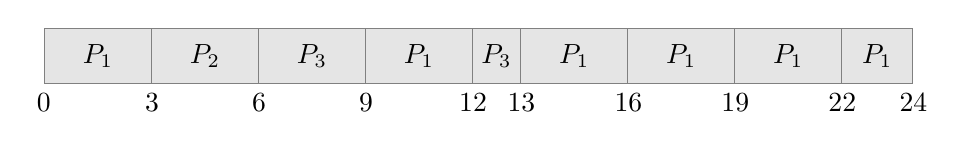
\begin{tikzpicture}[node distance=-0.5pt]
  \node [gray box=4.5] (p1) {\(P_{1}\)};
  \node [gray box=4.5, right=of p1] (p2) {\(P_{2}\)};
  \node [gray box=4.5, right=of p2] (p3) {\(P_{3}\)};
  \node [gray box=4.5, right=of p3] (p4) {\(P_{1}\)};
  \node [gray box=1.5, right=of p4] (p5) {\(P_{3}\)};
  \node [gray box=4.5, right=of p5] (p6) {\(P_{1}\)};
  \node [gray box=4.5, right=of p6] (p7) {\(P_{1}\)};
  \node [gray box=4.5, right=of p7] (p8) {\(P_{1}\)};
  \node [gray box=3, right=of p8] (p9) {\(P_{1}\)};

  \node [annotation] at (p1.south west) {0};
  \node [annotation] at (p1.south east) {3};
  \node [annotation] at (p2.south east) {6};
  \node [annotation] at (p3.south east) {9};
  \node [annotation] at (p4.south east) {12};
  \node [annotation] at (p5.south east) {13};
  \node [annotation] at (p6.south east) {16};
  \node [annotation] at (p7.south east) {19};
  \node [annotation] at (p8.south east) {22};
  \node [annotation] at (p9.south east) {24};
\end{tikzpicture}
\caption{Schedule with a time quantum of 3}
\end{figure}
\noindent Wait times:
\begin{itemize}
\item $P_{1}$: 7 time units
\item $P_{2}$: 3 time units
\item $P_{3}$: 9 time units
\end{itemize}
\noindent Average wait time = $19 / 3 = 6.33$ time units.
\n
However, a time quantum of 10 would result in a much longer average wait time.
\begin{figure}[H]
\centering
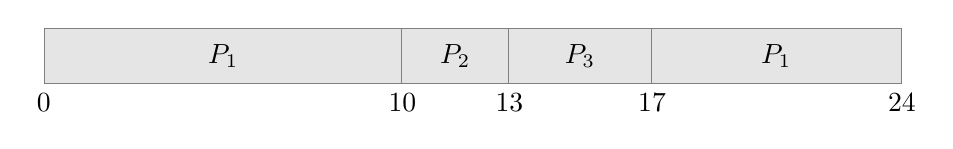
\begin{tikzpicture}[node distance=-0.5pt]
  \node [gray box=15] (p1) {\(P_{1}\)};
  \node [gray box=4.5, right=of p1] (p2) {\(P_{2}\)};
  \node [gray box=6, right=of p2] (p3) {\(P_{3}\)};
  \node [gray box=10.5, right=of p3] (p4) {\(P_{1}\)};

  \node [annotation] at (p1.south west) {0};
  \node [annotation] at (p1.south east) {10};
  \node [annotation] at (p2.south east) {13};
  \node [annotation] at (p3.south east) {17};
  \node [annotation] at (p4.south east) {24};
\end{tikzpicture}
\caption{Schedule with a time quantum of 10}
\end{figure}
\noindent Wait times:
\begin{itemize}
\item $P_{1}$: 7 time units
\item $P_{2}$: 10 time units
\item $P_{3}$: 13 time units
\end{itemize}
\noindent Average wait time = $30 / 3 = 10$ time units.
\n
It can be seen from the example how the choice of time quantum affects the waiting time, response time and number of context switches required. Round-robin is strong in cases where all processes bursts have similar lengths, or fairness is of greater importance to the system. For example in load balancing for parallel computation or time-sharing 

 
Changing the size of the time quantum affected the average waiting time, response time and number of context switches needed. as process 2 and 3 had to wait much longer before getting a chance to run. However, this comes at a trade-off of less context switches. With a quantum of 10, only 3 context switches were required, whereas with a quantum of 3, 8 context switches were required. 
\n
An issue with the simple round-robin scheduling approach is the long average waiting time. Given $n$ processes in the ready queue with a time quantum of $t$, each process only gets $t$ time to run every $nt$ time units and must wait at most $(n - 1) \times t$ before each turn. 
\n
Round-robin performs well for load balancing if the processes all have similar bursts times. 
\n
Some processes want/should have more share of the processor than others (concept for priority)
\n
Long queue leads to high response time and high turnaround time as a simple round-robin approach adds new processes to the tail of the queue, giving a response time of at most $(n - 1) \times t$ time units where $n$ is the number of processes in the queue and $t$ is the time quantum.
\section{Task 2 - Search for high performance schedules}

\subsection{Methodology}
A genetic algorithm was chosen as a means to explore the search space of binary schedules. Because of the large optimisation space of schedules, a genetic algorithm with mutation adds elements of randomness to help explore more of the search space compared to a hill climbing algorithm which can get easily stuck in local maxima. Furthermore, hill climbing with random restart will only try to explore another unrelated area of the search space for a maximum without taking into account the previous local maxima. With a genetic algorithm, the next generation is created based on the previous generation, so good schedules can be maintained and modified through each generation. The fitness function used to evaluated a schedule is the total time taken of the execution of that schedule from the output of the simulation. The less time taken, the fitter that individual. As a schedule is a binary string, this maps perfectly to a genetic chromosome, where each gene is a single bit.
\n
The genetic algorithm that was implemented follows three basic steps \cite{ga}:
\begin{enumerate}
\item \textbf{Selection} - Select parents to use for reproduction of next generation. The fitter the chromosome, the more likely it will be chosen for reproduction. \textbf{Elitism} is also implemented, keeping exact clones of the most fit individuals so the best schedules are not lost.
\item \textbf{Crossover} - Mix the genes of the parents to create two new child schedules.
\item \textbf{Mutation} - Genes (bits) of all child schedules have a chance to be mutated to increase diversity and prevent the algorithm from being stuck in a local maxima.
\end{enumerate}
\subsubsection{Selection}
A tournament selection method was used to select parents for reproduction. This method randomly selects a few chromosomes from the population, and chooses the most fit individual as the ``winner" of the tournament. Tournament selection was used for its simplicity and flexibility. The tournament size can be decreased to allow weaker individuals more chance to be selected for more diversity or increased to give them less chance for faster convergence. 
\n
The same individuals are allowed to be selected multiple times for reproduction for better convergence. It is also done so the randomness in the crossover and mutation stages do not lead to a complete loss of strong genes. Additionally, a small random number of elites are selected to be clone in each generation as part of \textbf{Elitism} to keep the fittest individuals. This is done to ensure the best schedules survive every generation as the effect of crossover and mutation on creating consistently better schedules is not known due to the size and complexity of the search space. The number of elites kept is randomised so the same elites are not kept every generation if the algorithm is at a local maximum.
\subsubsection{Crossover}
The simulator is deterministic, that is to say the same schedule will always take the same time to run. Additionally, if two schedules share the same initial $n$ bits, they will run identically until they differ. This means that where the bits change in the binary stream matters. Given a binary schedule, if the first few bits are modified, the rest of the schedule may be interpreted completely differently even if no other bits are modified. If only the last few bits are modified, then the schedule is only different at those last few bits. The crossover step for genetic algorithms is quite suited for this behaviour. The children created by the two parents will each contain the first $n$ bits from each parent and the rest from the other parent. If both parents were good schedules, this explores changing and mixing the second half of the schedule to potentially find an even better schedule without losing the good performance from the first half of the schedule. 
\begin{figure}[H]
\centering
\begin{tikzpicture}[
  node distance=+1em and +0pt,
  outer xsep=+0pt,
  outer ysep=+0pt
]
 \listset{chain name=p1,do={[s1]1,[s1]1,[s1]1,[s1]0,[s1]1,[s1]0,[s1]0,[s1]0,[s1]1,[s1]1,[s1]0,[s1]1,[s1]0,[s1]0,[s1]0,[s1]0}}
 
 \tikzset{every first on chain/.style={below=of \tikzpreviouschain-begin}}
 
 \listset{chain name=p2, do={[s2]0,[s2]0,[s2]1,[s2]1,[s2]1,[s2]1,[s2]0,[s2]1,[s2]1,[s2]1,[s2]0,[s2]0,[s2]1,[s2]1,[s2]1,[s2]0}}

 
 \listset{chain name=c1,do={[s1]1,[s1]1,[s1]1,[s1]0,[s1]1,[s1]0,[s1]0,[s1]0, [s2]1,[s2]1,[s2]0,[s2]0,[s2]1,[s2]1,[s2]1,[s2]0}}
   
 \listset{chain name=c2, do={[s2]0,[s2]0,[s2]1,[s2]1,[s2]1,[s2]1,[s2]0,[s2]1,[s1]1,[s1]1,[s1]0,[s1]1,[s1]0,[s1]0,[s1]0,[s1]0}}

 \draw[thick, dash pattern=on \pgflinewidth off \pgflinewidth]([yshift=1em]p1-8.north east) -- ([yshift=-1em]c2-8.south east);
 
 \node[below, yshift=-1em] at (c2-8.south east) {Crossover point};
 \node[right, xshift=1em] at (p1-16.east) {Parent 1};
 \node[right, xshift=1em] at (p2-16.east) {Parent 2}; 
 \node[right, xshift=1em] at (c1-16.east) {Child 1};
 \node[right, xshift=1em] at (c2-16.east) {Child 2};

\end{tikzpicture}
\caption{Example reproduction of children}
\label{fig:crossover}
\end{figure}
\noindent There is only one single crossover point in the implementation as more complicated crossover techniques would take less advantage of the deterministic behaviour of the simulator and schedule. The crossover point is chosen randomly for more diversity as the same individual can be chosen as a parent multiple times. 
\subsubsection{Mutation}
The mutation aspect of the algorithm will add diversity to the population, potentially changing a child schedule completely. This leads to a loss of a potentially good schedule, especially if the mutation occurred early and the parents were fit, but allows searching through more of the optimisation space to try and find even better schedules.
\begin{figure}[H]
\centering
\begin{tikzpicture}[
  node distance=+1em and +0pt,
  outer xsep=+0pt,
  outer ysep=+0pt
] 
  
 \listset{chain name=c1,do={[s1]1,[s3]0,[s1]1,[s1]0,[s3]0,[s1]0,[s1]0,[s1]0, [s2]1,[s2]1,[s2]0,[s2]0,[s2]1,[s2]1,[s2]1,[s2]0}}
   
 \tikzset{every first on chain/.style={below=of \tikzpreviouschain-begin}}   
   
 \listset{chain name=c2, do={[s2]0,[s2]0,[s2]1,[s2]1,[s2]1,[s2]1,[s2]0,[s2]1,[s1]1,[s3]0,[s3]1,[s1]1,[s1]0,[s3]1,[s1]0,[s1]0}}

 \node[right, xshift=1em] at (c1-16.east) {Child 1 with mutation};
 \node[right, xshift=1em] at (c2-16.east) {Child 2 with mutation};
\end{tikzpicture}
\caption{Children from figure \ref{fig:crossover} with mutation}
\label{fig:mutation}
\end{figure}
\noindent It is important to note that although the combination of selection, crossover and mutation can lead to a systematic way of searching for better schedules while taking into account previous strong genes and keeping the best individuals, the complexity of the search space and lack of understanding on how changes to the bits directly affect the time taken make the performance of genetic algorithm unpredictable. It could well be that randomly creating schedules is an easier and faster method to find the fastest schedule. 

\subsubsection{Parameters and other optimisations}

Optimise size of schedule as much as possible to prevent entire lower half being unused

- because we don't know how schedule affects time, unsure if crossover/selection/mutation strategies are suitable

- if schedule is too short, then the simulator will fail and return 0 for that fitness -> this allows removing potential bad schedules

\subsection{Experimentation}
The two benchmarks \texttt{sched-blackscholes_gen} and \texttt{sched-bodytrack_gen} are used in the experimentation. Initially, a na\"{i}ve experiment was run using arbitrary parameters to see how well the genetic algorithm performed after many generations. Afterwards, the experiment was improved by adjusting the parameters to improve diversity. The results of both experiments are later compared with the default weighted RNG scheduler and a completely random approach. 
\n

\subsubsection{Experiment 1}
In the first na\"{i}ve experiment, the following parameters were chosen:
\begin{itemize}
\item \textbf{Population size}: 25
\item \textbf{Chromosome length}: 100000
\item \textbf{Mutation probability per gene}: $\dfrac{1}{(l/10)}$ where $l$ is the length of the chromosome
\item \textbf{Crossover point}: Random
\item \textbf{Selection}: Tournament with 3 competitors
\end{itemize}
The population size was chosen as a size that was not too small or too large to start with. Fine tuning the population size for the specific task of finding a fast schedule will require more work, but starting with a medium sized population will give an indication as to whether this is too small or too large. A population that is too small will be stuck in a local maximum and unable to find better solutions, while a population that is too large would lead to a slow rate of convergence \cite{ga-size}.
\subsubsection{Experiment 2}
From the first experiment, it was noticed that the algorithm starts to stagnate quickly. After a few generations, either because of a lack of mutation or population size, a large portion of each generation end up with the same schedule and fitness with little diversity. To fix this issue, the population and mutation probability is increased to increase diversity. The larger population and higher mutation rate explores more of the search space, but leads to slower convergence. To be able to keep strong individuals with the increased population and mutation, the number of individuals used in the tournament selection is also increased.
\n
Increased mutation also due to local maxima. Perhaps crossover is not effective because if the schedule is good, only some portion of the top half of the binary is used, so low mutation rate where mutation happens in lower half has no effect.
\begin{itemize}
\item \textbf{Population size}: 40
\item \textbf{Chromosome length}: 100000
\item \textbf{Mutation probability per gene}: $\dfrac{1}{(l/100)}$
\item \textbf{Crossover point}: Random
\item \textbf{Selection}: Tournament with 5 competitors
\end{itemize}

\subsection{Results}

\begin{figure}[H]
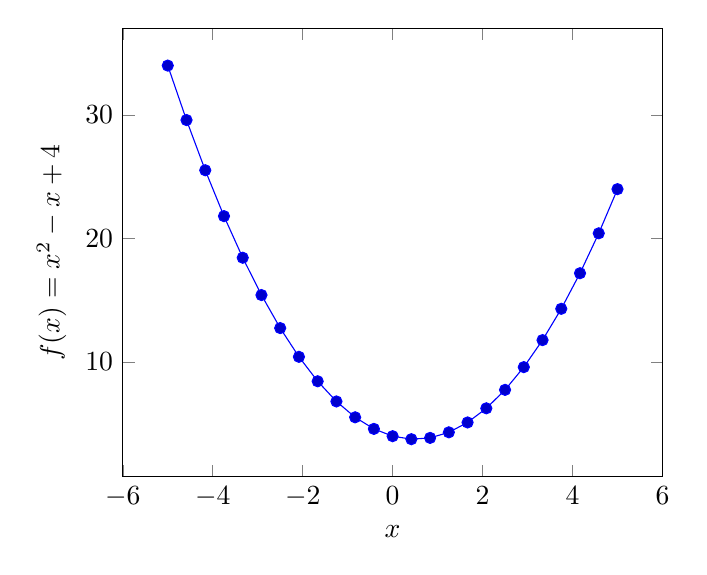
\begin{tikzpicture}
  \begin{axis}[ 
    xlabel=$x$,
    ylabel={$f(x) = x^2 - x +4$}
  ] 
    \addplot {x^2 - x +4}; 
  \end{axis}
\end{tikzpicture}
\end{figure}


- more time on genetic algorithm should tend to better result -> especially if given more diversity
- random gets faster schedule quicker, but less likely over time to find good schedule, whereas genetic algorithm guarantees good schedule over time as long as high diversity.
- ga can never/rarely get optimal schedule

\subsection{Evaluation}

\printbibliography

\end{document}



